\documentclass{beamer}
\usetheme{Copenhagen}
\setbeamertemplate{navigation symbols}{}

\usepackage[utf8]{inputenc}
\usepackage{chari}

\title{QR Preconditioner}
\author{Govind Chari}
\date{May 2023}
\institute{Univeristy of Washington}
\logo{
\includegraphics[width=1.8cm]{img/seal_black.pdf}\hspace*{8cm}~
\includegraphics[height=2cm]{img/ACL_logo.png}}

\begin{document}
\begin{frame}
    \titlepage
\end{frame}

\logo{}

\begin{frame}{Preconditioning}
    \begin{block}{Definition}
        Transforming a given problem into an equivalent problem that is more numerically stable or can be solved quicker
    \end{block}  
\end{frame}

\begin{frame}{Example}
    $$\min_{x} x_1^2 + 10x_2^2$$
    $$x_{k+1} = x_k - \gamma_k \nabla f(x_k)$$
    $$\gamma_k = \frac{\nabla f(x_k)^\top \nabla f(x_k)}{\nabla f(x_k)^\top P \nabla f(x_k)}$$
    \begin{center}
        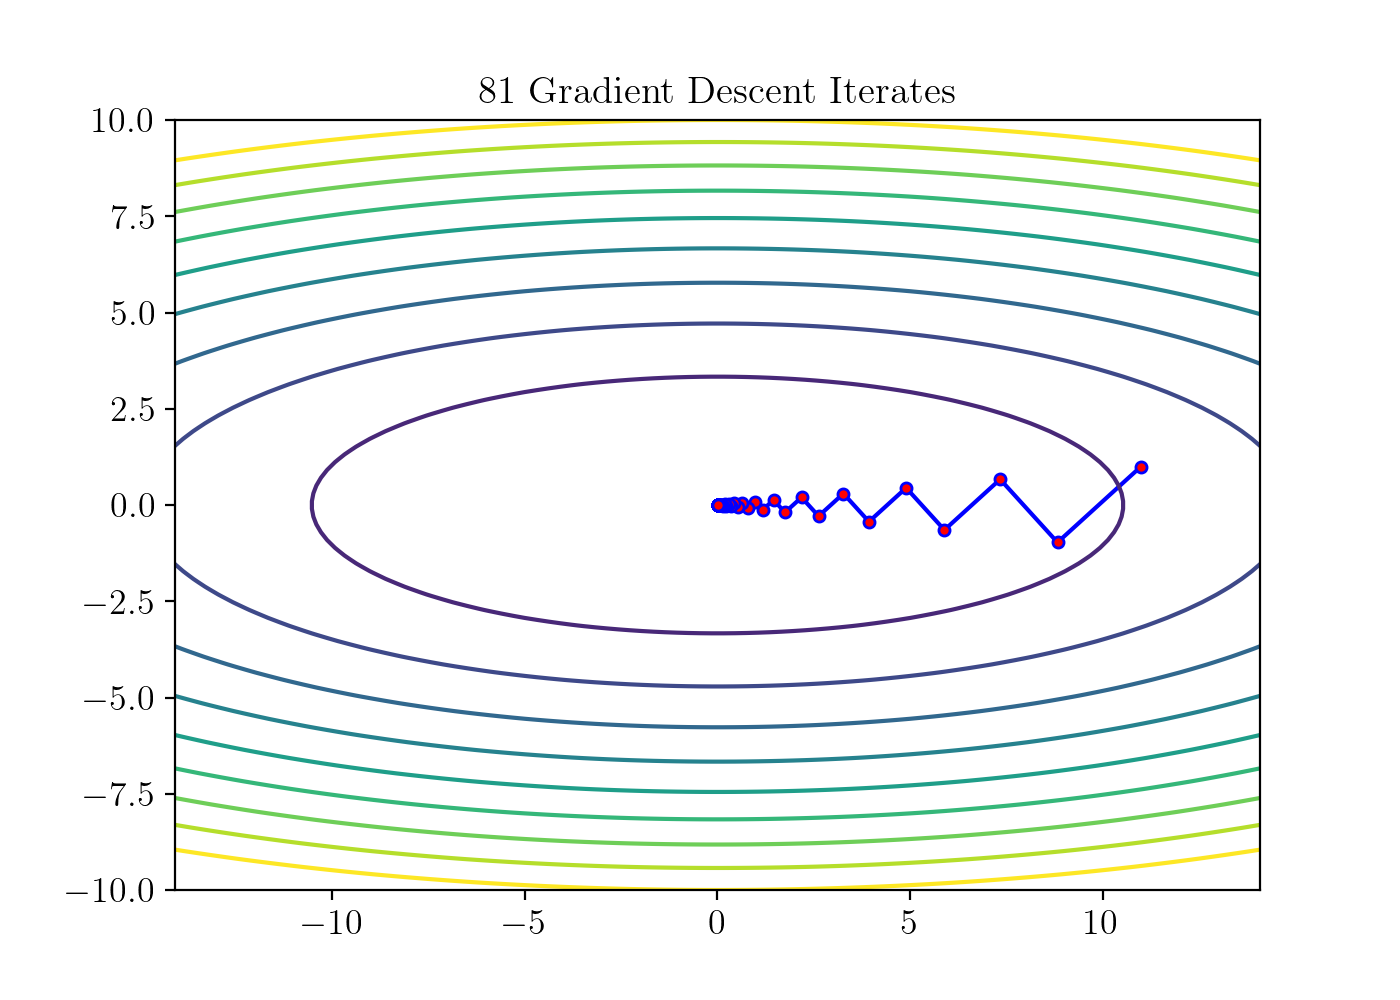
\includegraphics[width=7cm]{img/ill_conditioned.png}
    \end{center}
\end{frame}

\begin{frame}{Example}
    $$z_1 = x_1$$
    $$z_2 = \sqrt{10x_1}$$
    $$\min_{z} z_1^2 + z_2^2$$

    \begin{center}
        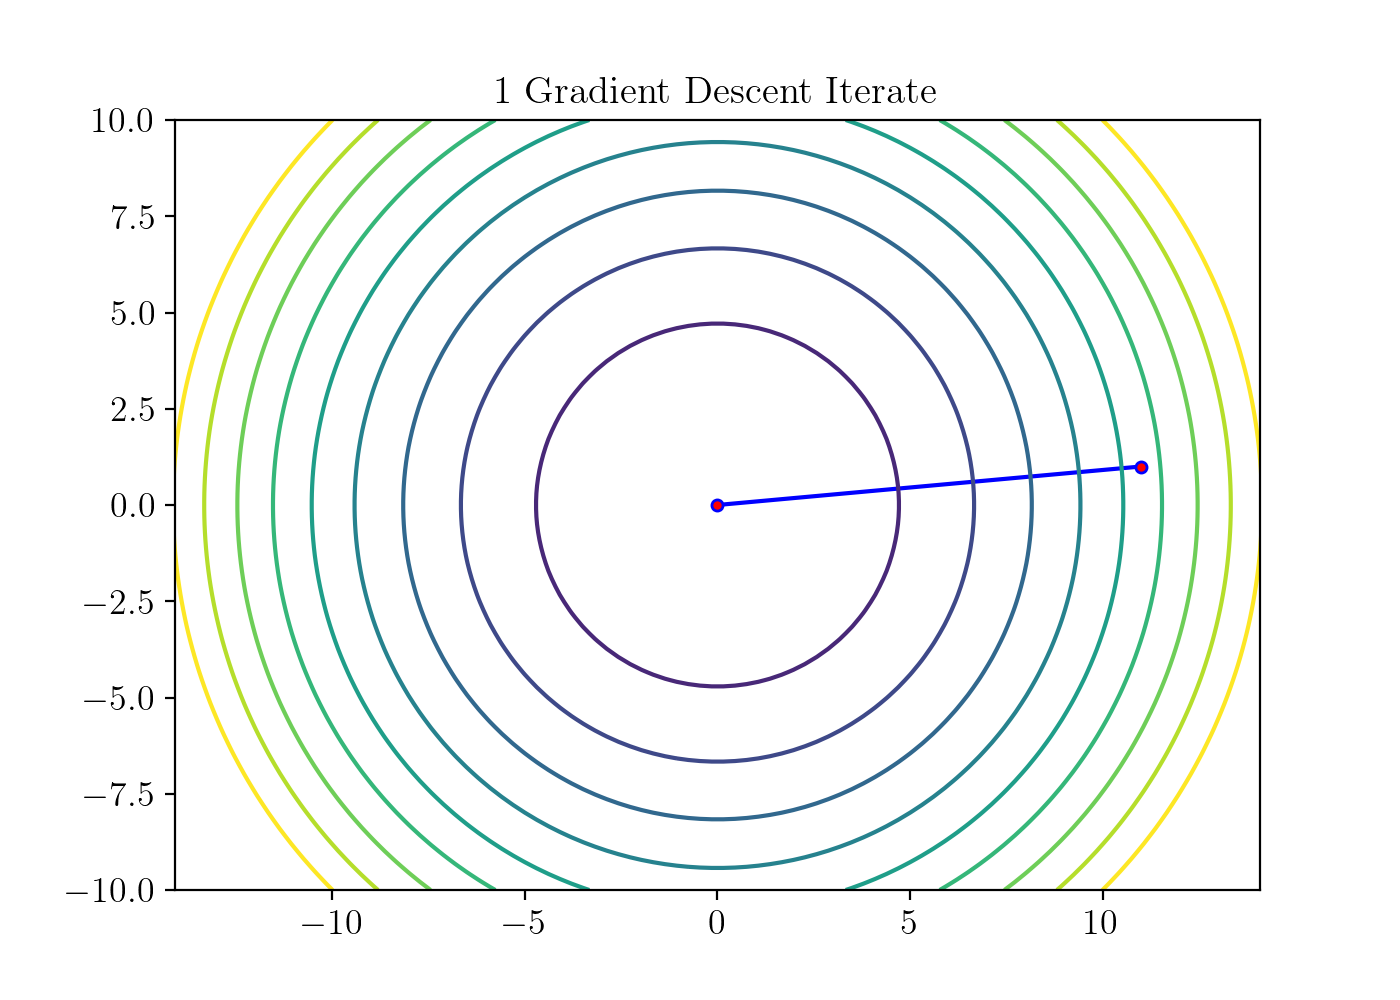
\includegraphics[width=7cm]{img/well_conditioned.png}
    \end{center}
\end{frame}

\end{document}